\section{Captura}
\paragraph{a}
Comando com o filtro de captura pretendido:
\begin{verbatim}
tcpdump -nn 'tcp[tcpflags] & tcp-push == tcp-push' and 'ip[2:2] < 128' > ssh.dump
\end{verbatim}

O resultado da captura é o seguinte:
\begin{verbatim}
11:00:59.019099 IP 170.2.0.33.41460 > 192.180.30.44.22: Flags [P.], seq 3235348810:3235348854, ack 1796210900, win 288, options [nop,nop,TS val 2288580 ecr 2411765], length 44
11:00:59.503156 IP 170.2.0.33.41460 > 192.180.30.44.22: Flags [P.], seq 44:80, ack 93, win 288, options [nop,nop,TS val 2289064 ecr 2470611], length 36
11:00:59.503611 IP 192.180.30.44.22 > 170.2.0.33.41460: Flags [P.], seq 93:129, ack 80, win 340, options [nop,nop,TS val 2471095 ecr 2289064], length 36
11:00:59.503638 IP 192.180.30.44.22 > 170.2.0.33.41460: Flags [P.], seq 129:173, ack 80, win 340, options [nop,nop,TS val 2471095 ecr 2289064], length 44
11:01:00.504865 IP 192.180.30.44.22 > 170.2.0.33.41460: Flags [P.], seq 173:217, ack 80, win 340, options [nop,nop,TS val 2472096 ecr 2289064], length 44
11:01:01.505841 IP 192.180.30.44.22 > 170.2.0.33.41460: Flags [P.], seq 217:261, ack 80, win 340, options [nop,nop,TS val 2473097 ecr 2290066], length 44
11:01:02.506759 IP 192.180.30.44.22 > 170.2.0.33.41460: Flags [P.], seq 261:305, ack 80, win 340, options [nop,nop,TS val 2474098 ecr 2291067], length 44
11:01:03.507958 IP 192.180.30.44.22 > 170.2.0.33.41460: Flags [P.], seq 305:349, ack 80, win 340, options [nop,nop,TS val 2475099 ecr 2292068], length 44
11:01:04.508887 IP 192.180.30.44.22 > 170.2.0.33.41460: Flags [P.], seq 349:393, ack 80, win 340, options [nop,nop,TS val 2476100 ecr 2293069], length 44
11:01:05.509815 IP 192.180.30.44.22 > 170.2.0.33.41460: Flags [P.], seq 393:437, ack 80, win 340, options [nop,nop,TS val 2477101 ecr 2294070], length 44
11:01:06.510972 IP 192.180.30.44.22 > 170.2.0.33.41460: Flags [P.], seq 437:481, ack 80, win 340, options [nop,nop,TS val 2478102 ecr 2295071], length 44
11:01:07.511956 IP 192.180.30.44.22 > 170.2.0.33.41460: Flags [P.], seq 481:533, ack 80, win 340, options [nop,nop,TS val 2479103 ecr 2296072], length 52
11:01:07.881220 IP 170.2.0.33.41460 > 192.180.30.44.22: Flags [P.], seq 80:116, ack 533, win 288, options [nop,nop,TS val 2297442 ecr 2479103], length 36
11:01:07.881675 IP 192.180.30.44.22 > 170.2.0.33.41460: Flags [P.], seq 533:569, ack 116, win 340, options [nop,nop,TS val 2479473 ecr 2297442], length 36
11:01:07.881775 IP 192.180.30.44.22 > 170.2.0.33.41460: Flags [P.], seq 569:605, ack 116, win 340, options [nop,nop,TS val 2479473 ecr 2297442], length 36
11:01:07.881861 IP 192.180.30.44.22 > 170.2.0.33.41460: Flags [P.], seq 605:665, ack 116, win 340, options [nop,nop,TS val 2479473 ecr 2297442], length 60
11:01:07.882171 IP 192.180.30.44.22 > 170.2.0.33.41460: Flags [P.], seq 665:717, ack 116, win 340, options [nop,nop,TS val 2479473 ecr 2297443], length 52
\end{verbatim}

\begin{figure}[h]
\centering
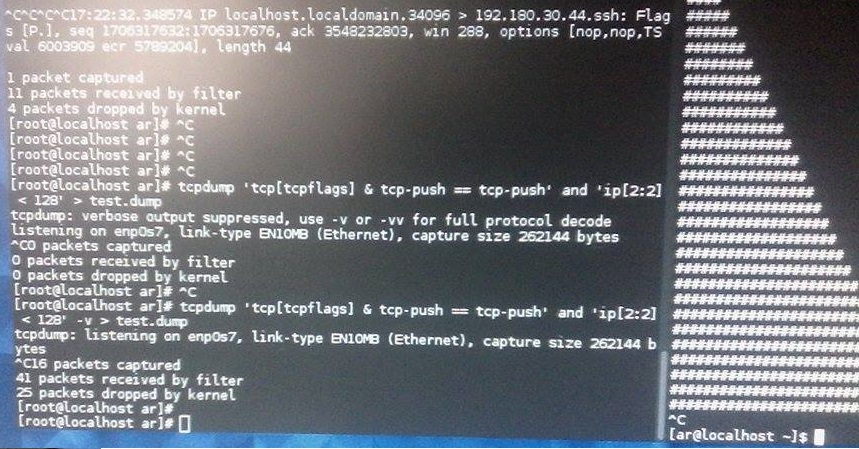
\includegraphics[width=0.7\textwidth]{3_a_filtro.png}
\label{fig:filtro}
\caption{Teste do filtro utilizado.}
\end{figure}

\begin{figure}[h]
\centering
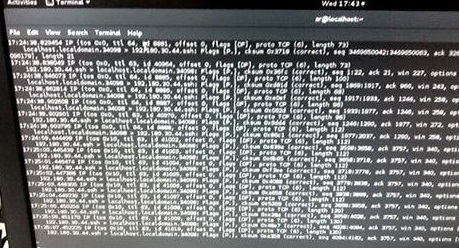
\includegraphics[width=0.7\textwidth]{3_a_resultado_do_tcpdump.png}
\label{fig:tcpdump}
\caption{Resultado do filtro de captura.}
\end{figure}

\paragraph{b}
Filtro de visualização pretendido:
\begin{verbatim}
tcp.flags.push == 1 && ip.len < 128
\end{verbatim}
Na figura a baixo, podemos ver o resultado da captura, no \emph{wireshark}, usando este filtro.

\begin{figure}[h]
\centering
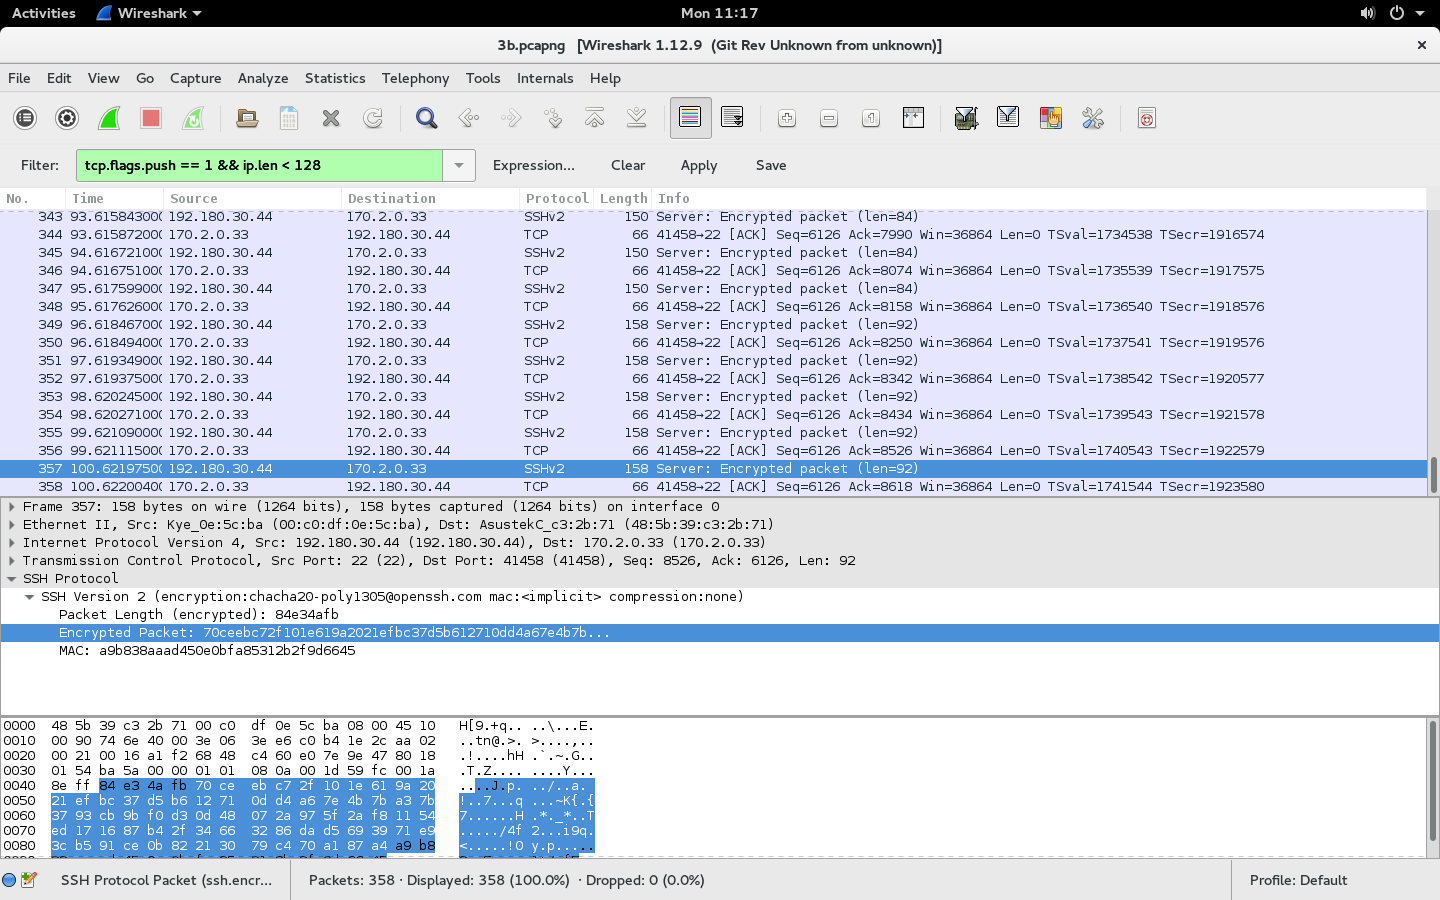
\includegraphics[width=0.7\textwidth]{3_b_screenshot.png}
\label{fig:wireshark}
\caption{Resultado do filtro de visualização do \emph{wireshark}.}
\end{figure}

\paragraph{c}
Para calcular o comprimento de um pacote IP subtrai-se o seu tamanho total (cabeçalho + dados), encontrado nos bytes 2 a 3 (indexado a 0), pelo comprimento do próprio cabeçalho, encontrado no primeiro byte, nos últimos 4 bits (mais à direita).